%
%  untitled
%
%  Created by Saulius Archipovas on 2013-02-07.
%  Copyright (c) 2013 __MyCompanyName__. All rights reserved.
%
\documentclass[]{article}

% Use utf-8 encoding for foreign characters
\usepackage[utf8]{inputenc}

% Setup for fullpage use
\usepackage{fullpage}

% Uncomment some of the following if you use the features
%
% Running Headers and footers
%\usepackage{fancyhdr}

% Multipart figures
%\usepackage{subfigure}

% More symbols
%\usepackage{amsmath}
%\usepackage{amssymb}
\usepackage{latexsym}

% Surround parts of graphics with box
\usepackage{boxedminipage}

% Package for including code in the document
\usepackage{listings}

% If you want to generate a toc for each chapter (use with book)
\usepackage{minitoc}

% This is now the recommended way for checking for PDFLaTeX:
\usepackage{ifpdf}

%\newif\ifpdf
%\ifx\pdfoutput\undefined
%\pdffalse % we are not running PDFLaTeX
%\else
%\pdfoutput=1 % we are running PDFLaTeX
%\pdftrue
%\fi

\ifpdf
\usepackage[pdftex]{graphicx}
\else
\usepackage{graphicx}
\fi
\title{A LaTeX Article}
\author{  }

\date{2013-02-07}

\begin{document}

\ifpdf
\DeclareGraphicsExtensions{.pdf, .jpg, .tif}
\else
\DeclareGraphicsExtensions{.eps, .jpg}
\fi

\maketitle


\begin{abstract}
	In diese Ausarbeitung werden Saulius, Thorben und Dima euch was über design for mobile kontext erzählen.
\end{abstract}

\section{Introduction}
%!TEX root = ../abgabe.tex

\section{Einführung}

Geschrieben von: \textbf{Dmytro Kozha}
\newline


In diesem Kapitel werden notwendige Kenntnisse zum Verständnis dieser Arbeit  eingeführt. Zunächst werden die wesentlichen Begriffe „mobiler Kontext“ und „Mobilgerät“ erklärt. Anschließend  werden verschiedene Eingabe- und Ausgabemöglichkeiten in den Mobilgeräten vorgestellt und auf die Schwierigkeiten, mit denen ein Designer konfrontieren muss, eingegangen.
\subsection{Was ist mobiler Kontext} % (fold)
\label{sub:was_ist_mobiler_kontext}
Bevor wir über das Design für mobilen Kontext sprechen, müssen wir zuerst klar stellen, was ein "mobiler Kontext" bedeutet. In dem Buch "The Mobile Frontier: A Guide for Designing Mobile Experiences“ beschreibt die Autorin, Rachel Hinman, ein Experiment, das im 2006 von einer Forschungsgruppe durchgeführt wurde und den Begriff des mobilen Kontext definiert. Eine Gruppe von Versuchspersonen wurde gebeten, die Orte zu fotografieren, an denen sie ihre Mobilgeräte nutzen. Die Forscher hofften, dass nach einer Analyse dieser Aufnahmen sie die grundlegenden Prinzipien des mobilen Kontexts bestimmen können. Nach einer Woche erhielten sie eine hohe Anzahl an Fotos von vollkommen unterschiedlichen Orten und Situationen, siehe Abbildung~\ref{fig:studie}.\cite{mobileFrontier}

 \begin{figure}[h]
 \centering
 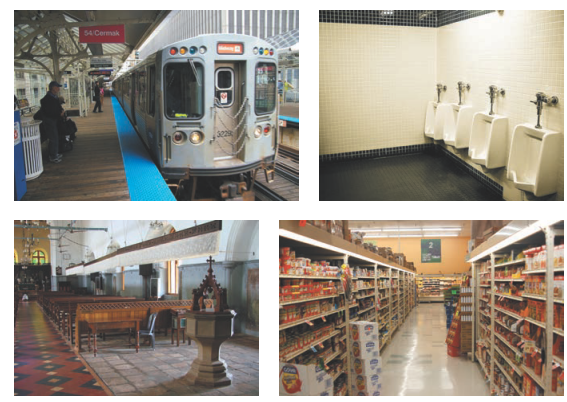
\includegraphics[height=0.25\textheight]{img/studie.png}
 \caption{Fotoaufnahmen der Versuchspersonen}\label{fig:studie}
\end{figure}

Die Fotos wurden unterwegs auf der Straße, im Supermarkt, im Bus oder im Zug, sowie auch an unerwarteten Orten, wie in einem Restaurant, im Schlafzimmer und sogar in einer Kirche geschossen. Selbst nach einer langen Sortierung, Kategorisierung und Analyse konnten sie dennoch kein Muster für den "mobilen Kontext" erkennen. Daraufhin kamen sie zu der Definition "Mobile context = anywhere and everywhere", was auf Deutsch übersetzt bedeutet: „mobiler Kontext“ ist immer und überall. Meiner Meinung nach ist das eine gute Bezeichnung dafür. Da im Vergleich zu der Interaktion mit dem herkömmlichen PC, geschieht die Interaktion im mobilen Kontext mitten im Leben des Benutzers. Verschiedene Mobilgeräte wie z.B. Smartphones  begleiten den Nutzer von morgens bis abends, oft bis ins Bett. Und die Aufgabe des Designers ist, das zu berücksichtigen und den Nutzern gute Bedienbarkeit anzubieten.

% subsubsection was_ist_mobiler_kontext (end)
\subsection{Mobilgeräte} % (fold)
\label{sub:mobile_ger_te}
Es gibt keine einheitliche und spezifizierte Definition von dem Begriff „Mobilgerät“. Man kann das Mobilgerät auf verschiede Arten und Weisen definieren. Die Definition kann hinsichtlich der Dienste oder dem Niveau der Funktionalität des Mobilgeräts bestimmt werden. Die folgenden Aussagen gelten allgemein: das Mobilgerät ist ein tragbares Endgerät und zur mobilen Verwendung gedacht.  Häufig werden unter dem Begriff Handys, Smartphones, Tablet Computers und Personal Digital Assistants (PDAs) zusammengefasst. Außerdem umfasst der Begriff  tragbare media player (MP3-Player), E-Book-Lesegeräte, tragbare Spielkonsolen (wie Nintendo DS, PSP), mobile Navigationssysteme und tragbare Fernsehgeräte. Es existieren auch Lösungen, die für spezielle Anwendungsgebiete geschaffen wurden, wie z.B. Wearable computing. 

 \begin{figure}[h]
 \centering
 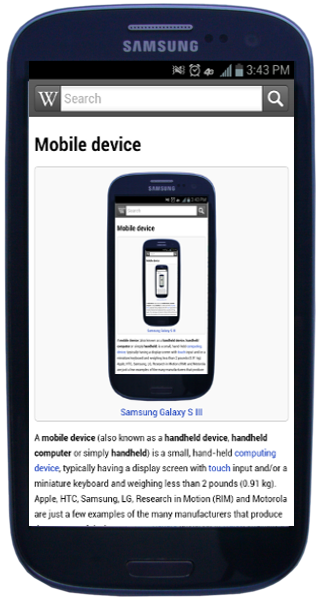
\includegraphics[height=0.25\textheight]{img/Samsung_Galaxy_S_III_Pebble_Blue_WikiWikipedia.png}
 \caption{Samsung Galaxy S3}\label{fig:galaxys3}
\end{figure}

Da heutzutage der Mobilität eine große Bedeutung zusteht, steigt die Popularität des Mobilgerätes in der Bevölkerung und es wird von verschiedenen Personen zu verschieden Zwecken eingesetzt.  Mit der Entwicklung der Technologien kommen auch immer mehr universale Mobilgeräte auf den Markt, die zur Kommunikation, Navigation und Unterhaltung gleichzeitig genutzt werden können, siehe Abbildung~\ref{fig:galaxys3}. 

% subsection mobile_ger_te (end)

\subsection{Einschränkungen in mobilen Kontexten} % (fold)
\label{sub:einschr_nkungen_in_mobilen_kontexten}
Bei der Entwicklung des Designs für die Mobilgeräte, stößt der Designer, laut Kuo-Ying Huang \cite{challhcimd} auf Probleme verschiedener Art, die die Hardware und die Software betreffen. 
Wie bereits erwähnt, gilt das für die Mobilgeräte das Prinzip "mobiler Kontext- immer und überall". Aus dem Grund spielt die Mobilität eine wichtige Rolle und zieht Einschränkungen bezüglich ihrer Größe und des Gewichts nach sich, was wiederum Hardware Einschränkungen zur Folge hat. Kuo-Ying Huang \cite{challhcimd} unterscheidet zwischen drei Arten der Hardware-Einschränkungen: begrenzte Eingabemöglichkeiten, begrenzte Ausgabemöglichkeiten und Design für Mobilität.

% subsection einschr_nkungen_in_mobilen_kontexten (end)

\subsubsection{Begrenzte Eingabemöglichkeiten} % (fold)
\label{ssub:einschr_nkungen_in_mentalen_bereich}
Die weitverbreitete und grundlegende Eingabemöglichkeiten für Mobilgeräte auf dem Markt sind zurzeit: Tastatur, Touchscreen und Trackball.

Die Tastatur

Die Tastatur ist derzeit die Hauptmethode für Texteingabe.  Beim Drücken einer Taste, ermöglicht sie dem Benutzer die Eingabe von Symbolen, die Ausführung einer Aktion oder die Navigation der Menüpunkte. Leider ist sie in ihrer Standardgröße für Mobilgeräte nicht geeignet. Das Design der Tastatur kann zu einer der schwierigsten Aufgabe werden. Der Mangel an Platz des Mobilgerätes zwingt den Designer nach alternativen Lösungen zu suchen. Eine solche Lösung ist eine Telefontastatur mit Buchstaben,siehe Abbildung~\ref{fig:tastatur}. 

 \begin{figure}[h]
 \centering
 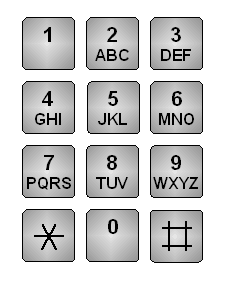
\includegraphics[height=0.25\textheight]{img/Tastatur_ITU-T-E161_4x3.png}
 \caption{Telefontastatur mit Buchstaben}\label{fig:tastatur}
\end{figure}

Bei dieser Tastatur werden Buchstaben auf die zehn Zifferntasten verteilt. Man muss auf eine Taste bis zu viermal drücken, um einen Buchstaben zu treffen. Die Geschwindigkeit bei den kürzeren Texten (z.B. Kurznachrichten) war akzeptabel, aber bei den größeren Texten leider nicht.  Für Wearable Computing werden auch interessante Konzepte weiterentwickelt, wie z.B. die Akkordtastatur. Das ermöglicht dem Benutzer Symbole oder Befehle bei gleichzeitigen drücken der Tasten einzugeben,siehe Abbildung~\ref{fig:twiddler}. 

 \begin{figure}[h]
 \centering
 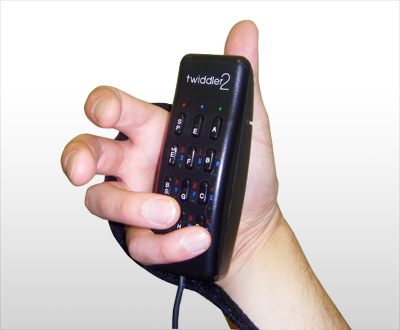
\includegraphics[height=0.25\textheight]{img/twiddler.jpg}
 \caption{Twiddler}\label{fig:twiddler}
\end{figure}

Man könnte das mit dem Klavierspielen vergleichen. Vielzahl von Kombinationen aus einer kleinen Anzahl von Tasten, ermöglicht die Eingabe mit einer Hand, während die andere frei bleibt. Ein anderer Vorteil ist dadurch, dass die Größe dieser Tastatur geringer als die der Standarttastatur sein kann. Allerdings muss der Benutzer mehr Kombinationen erlernen, was als ein Nachteil gesehen werden kann.


Der Touchscreen

Der Touchscreen ist eine gute Alternative für die Tastatur und ermöglicht dem Nutzer tippen auf virtuelle Tastatur. Jedoch treten bei ihrer Benutzung auch Schwierigkeiten auf. Im Falle eines zu kleinen Bildschirmes sieht der Benutzer bei der Eingabe nicht die graphischen Elemente, das sogenannte " fat-finger syndrome".  Um dies zu vermeiden, gibt es auch verschiedene Konzepte.

 \begin{figure}[h]
 \centering
 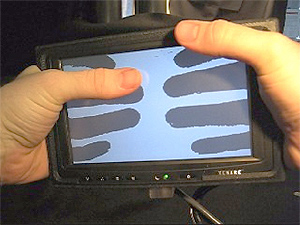
\includegraphics[height=0.25\textheight]{img/lucidtouch.jpg}
 \caption{The LucidTouch prototype}\label{fig:lucid}
\end{figure}

Eines davon ist LucidTouch,siehe Abbildung~\ref{fig:lucid} \cite{lucidtouch}, das ist ein Eingabegerät, das es dem Benutzer ermöglicht, die Anwendungen zu steuern, indem er die Rückseite des Gerätes berührt, so dass die Vorderseite nicht von den Fingern verdeckt wird. Die Grundidee dabei ist, dem Benutzer die Illusion von Pseudo-Transparenz zu geben. LucidTouch unterstützt auch multi-toch input, was die 10 Fingereingabe ermöglicht. Auch Forschungen haben ergeben, dass viele Benutzer gerne mit der Rückseite ihres Geräts agieren.

Der Trackball

Der Trackball wird hauptsächlich zur Navigation eingesetzt, aber auch zur Ausführung von Aktionen, durch das Drücken darauf. Der Vorteil des Trackballs ist, dass man nur einen Finger benötigt, um horizontal und vertikal im Menu zu navigieren. Leider zur Texteingabe ist er schlecht geeignet.
Außer obengenannten Eingabemöglichkeiten gibt’s auch neue Techniken, wie z.B. Scpracheingabe. Dafür wird ein Mikrofon verwendet und spezielle Spracherkennungssoftware. Der Nutzer spricht in das Mikrofon und die gesprochenen Wörter und Sätze werden in Text oder Befehle konvertiert. Spracherkennung  gehört zu den schwierigsten Aufgaben der Signalverarbeitung. Gesprochene Sprache hat einen individuellen Charakter und verschiedene Menschen sprechen gleiche Sätze auf eigene Art und Weise. Ein Spracherkennungsprogramm sollte diese Äußerungen als gleich erkennen. Für Mobilgeräte gibt’s zwar schon einige gute Lösungen, wie z.b. Google Voice Search 
\footnote{http://www.google.com/mobile/voice-search/}, Siri Personal Assistent \footnote{http://www.apple.com/ios/siri/} oder Vlingvo \footnote{http://www.vlignvo.com}. Leider meistens davon benötigen eine Internetverbindung, was nicht immer möglich ist.



% subsubsection einschr_nkungen_in_mentalen_bereich (end)

\subsubsection{Begrenzte Ausgabemöglichkeiten} % (fold)
\label{ssub:einschr_nkungen_in_bedienung}

Der Bildschirm


Es existieren eine Menge verschiedener Ausgabemöglichkeiten für Mobilgeräte. Ein Bildschirm ist eine der grundlegendsten davon. Um die passende Bildschirmgröße zu finden, braucht man viel Zeit und Erfahrung. Ein großer Bildschirm ist gut, da er viel Platz bietet, allerdings auch Mobilitätsprobleme mit sich bringt. Außerdem verbraucht ein großer Bildschirm offensichtlich mehr Strom, als ein kleiner Bildschirm derselben Art, was zu öfteren Aufladungen führt. 

 \begin{figure}[h]
 \centering
 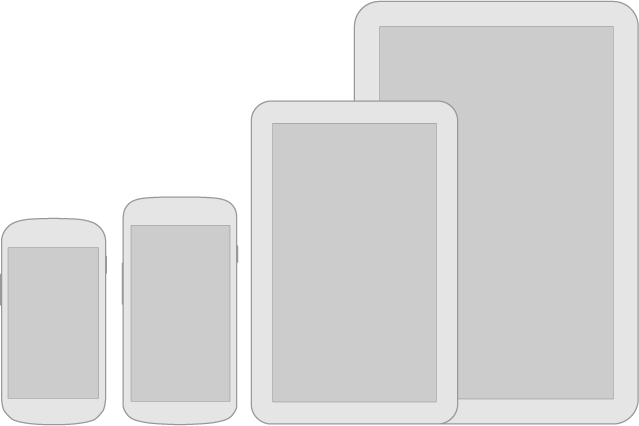
\includegraphics[height=0.25\textheight]{img/devices_displays_main.png}
 \caption{Verschiedene Bildschirme}
\end{figure}

Die Audio-Anlage und Vibration

Die Audio-Ausgabe ist eine weitere, oft verwendete Ausgabemöglichkeit für Mobilgeräte. Eine eingegangene Nachricht kann durch ein Ton-Singal in Verbindung mit grafischen Elementen und Text eine gute Interaktion zwischen Benutzer und Endgerät darstellen. In Mobilgeräten werden kleine und nicht leistungsstarke Lautsprecher eingesetzt. Das hat zur Folge, dass man beim großen Lärm eine wichtige Nachricht oder ein Ereignis verpassen kann. Eine gute Alternative ist eine Vibrationsfunktion. Im Mobilgerät wird ein kleiner Elektromotor eingebaut, der eine Welle antreibt. An der Welle hängt ein halber Zylinder und weil der Zylinder nur halb ist, hat er eine Unwucht, die bei schneller Drehung zu einer Vibration führt.


% subsubsection einschr_nkungen_in_bedienung (end)

\subsubsection{Design für Mobilität} % (fold)
\label{ssub:weiterf_hrung}

Da die Mobilgeräte immer und überall eingesetzt werden, entsteht das wichtigste Problem der Mobilität nämlich die Stromversorgung. Alle Hersteller wollen Akkus leistungsfähiger machen, leider sind sie nicht weit gekommen. Man kann mit einem Smartphone zurzeit nur ein Tag intensiv arbeiten. Es gibt zwar einige Verbesserungen bei den Akkus und sie konnten mithalten, aber durch die zusätzliche Technik, die größeren Bildschirme, die schnellen Netze und Prozessoren wird es wieder aufgezehrt.\cite{ndrarticle}

% subsubsection weiterf_hrung (end)
\section{Design Tips}

Written by: Saulius
%!TEX root = ../abgabe.tex

\section{Redesign von ''AutoTrader''}

Geschrieben von: \textbf{Hans-Thorben Juilfs}
\newline

In dieser Sektion geht es um ein Fallbeispiel. Das Re-Design und die Entstehung dessen werden beleuchtet und erklärt. Außerdem wird im Folgenden auf einzelne, wichtige Komponenten in der Planung des Designs, sowie der Vorgehensweise eingegangen. Zunächst wird es um die UI-Komponenten(User Interface) gehen.\\

Das Fallbeispiel ist das Re-Design von der iOS app ''AutoTrader'' für Android. Wir haben uns entschieden die im Referat vorgestellte Navigationssoftware nicht noch einmal zu beschreiben, sondern auf eine etwas aktuellere Software zurückzugreifen, um neuere Designaspekte deutlicher ausleuchten zu können.\\

Dabei werden einige Beispiele aufgeführt, die bebildert beschrieben werden und so den Zugang erleichtern.\\

Die vorliegenden Informationen beruhen auf dem Buch ''Android Design Patterns: Interaction Design Solutions for Developers'' von Greg Nudelman\\


\subsection{Logo-Design}
\label{sub:logodesign}
Zunächst wird das Logo und das ensprechende Re-Design beschrieben:\\

\begin{figure}[h]
 \centering
 
\includegraphics[height=0.10\textheight]{img/logo.png}
 \caption{Re-Design des Logos}
 \label{fig:logo}
\end{figure}

Ein Logo wird nach Vorschrift von Apple Inc. immer viereckig, mit abgerundeten Ecken dargestellt. Diese Limitation liegt für Android App-logos nicht vor. Hier wird mehr künstlerische Freiheit gegeben. Um dies zu verdeutlichen wird einfach ein Teil des iOS App-logos genommen und als neues Logo angepasst(siehe Abbildung~\ref{fig:logo}).(\cite{AndroidDesignPatterns} Seite 5)

\subsection{Redesign}
\label{sub:actionbars}

\subparagraph{Vorher}
\label{subp:vorher}
Ersteinmal beschreibt der Autor Greg Nudelman das Aussehen der App bevor das Design angepasst wurde. Hierbei wird aufgezeigt, dass ein großer Knopf mit der Aufschrift ''Settings'' nichts an dem angestammten Platz in der oberen rechten Ecke des Bildschirmes zu suchen hat, da es sich dabei um eine der wichtiges Positionen auf der GUI handelt. Hinzukommt, dass der Knopf keine Einstellungen zeigt, wenn er ausgelöst wurde, sondern lediglich eine ''Anwalts''-Seite zeigt, auf der sich ''Privacy Policy'', ''Visitor Agreement'' und ein Knopf mit der Aufschrift ''Email-Feedback'' befinden(\cite{AndroidDesignPatterns} Seite 6).\\

\begin{figure}[h]
 \centering
 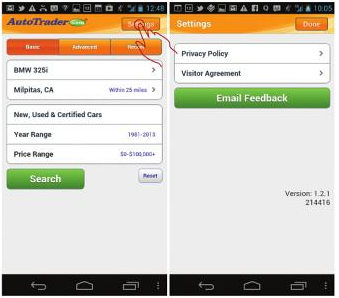
\includegraphics[height=0.40\textheight]{img/Design1.png}
 \caption{Design der GUI1}
 \label{fig:design1}
\end{figure}

Da der ''Settings''-Knopf so einen wichtigen Platz einnimmt, werden wichtigere Funktionen, wie ''Find cars'', ''Find dealer'' oder ''Scan \& Find'' in den Hintegrund gedrängt und sind in einer einem älteren Android nachempfundenen navigation bar menu versteckt. Beides wird in Abbildung~\ref{fig:design1} und Abbildung~\ref{fig:design2} durch eine rote Hand angezeigt.

\begin{figure}[h]
 \centering
 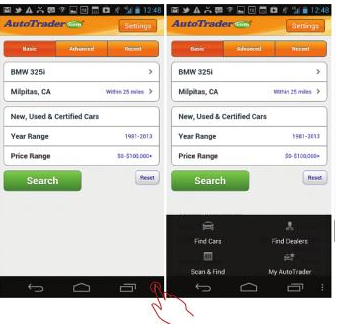
\includegraphics[height=0.40\textheight]{img/Design2.png}
 \caption{Design der GUI2}
 \label{fig:design2}
\end{figure}

\subparagraph{Nachher}
\label{subp:nachher}
Anschließend werden Schritte des Redesigns beschrieben. Zunächst geht Nudelman auf das Umgestalten der o.b. Aspekte, insbesondere den ''Settings''-Knopf und die verstecktion Funktionen ein. In Abbildung~\ref{fig:design3} sind folgende Änderungen zu finden: \\
\begin{itemize}
\item Die Beschriftung des o.g. Knopfes wurde entfernt und durch ein Symbol erseltzt, um ikonische Sprache zu verwenden(\cite{AndroidDesignPatterns} Seite 7). Dies erleichtert die Lokalisation für andere Kulturen, weil nicht übersetzt werden muss. 
\item Der ehemalige Inhalt der navigation bar wurde in die Action bar am oberen Bildschirmrand verschoben und ist so leichter zu finden(\cite{AndroidDesignPatterns}) Seite 7. Dies hilft insbesondere Menschen, welche Schwierigkeiten mit dem Durchsuchen des Bildschirmes nach Funktionen haben. Dabei kann es sich um Blindheit bzw. Sichteinschränkungen oder auch andere, vielleicht psychische Schäden oder Einschränkungen handeln, die ein einfaches Zurechtfinden erschweren.
\end{itemize}

\begin{figure}[h]
 \centering
 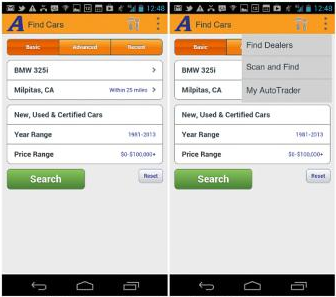
\includegraphics[height=0.40\textheight]{img/Design3.png}
 \caption{Re-Design der GUI1}
 \label{fig:design3}
\end{figure}

Wie Nudelman sagt, wurden aber wichtige Aspekte noch nicht beachtet, während der ersten Umgestaltung. Diese sind:
\begin{itemize}
\item Die Option ''Settings'' ist nicht hilfreich, steht aber durch die prominente Platzierung auf der GUI immernoch über den Funktionen, die im Dropdown menu zu finden wären. Ein Benutzer kommt vermutlich schnell zu dem Schluss, dass die versteckten Funktionen noch weniger hilfreich, als die prominent angeordneten sind und ruft sie daher garnicht erst auf.
\item Die wichtigen Optionen werden nicht auf Anhieb gefunden und erfordern daher Suchkapazitäten, die durch den ersten genannten Punkt demotiviert werden(\cite{AndroidDesignPatterns} Seite 8) oder eventuell durch Benutzer mit mentalen oder physischen Herrausforderungen garnicht aufgebracht werden können.
\end{itemize}

Diese Aspekte wurden in Abbildung~\ref{fig:design4} beachtet und durch erneute Umgestaltung verwirklicht. Wichtige Funktionen (''Find Dealers'' und ''My AutoTrader'') wurden in die Action bar aufgenommen und ''Settings'' wurde in das Dropdownmenu verschoben(Siehe Abbildung~\ref{fig:design4}).

\begin{figure}[h]
 \centering
 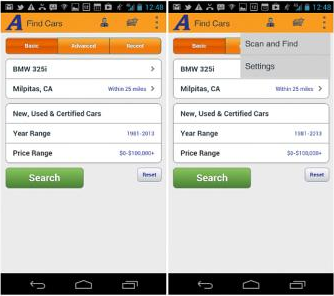
\includegraphics[height=0.40\textheight]{img/Design4.png}
 \caption{Re-Design der GUI2}
 \label{fig:design4}
\end{figure}

\subparagraph{Tabs}
\label{sub:tabs}

\begin{figure}[h]
 \centering
 
\includegraphics[height=0.25\textheight]{img/tabs.png}
 \caption{Re-Design der Tabs}
 \label{fig:tabs}
\end{figure}

\bibliographystyle{plain}
\bibliography{sauliusBib}
\end{document}
